\documentclass{article}

\usepackage{iclr2026_conference,times}
\usepackage{microtype}
\usepackage{amsmath,amssymb,amsthm}
\usepackage{booktabs}
\usepackage{xcolor}
\usepackage{graphicx}
\usepackage[labelsep=space]{caption}
\usepackage{tikz}
\usetikzlibrary{arrows.meta,calc,fit,positioning}
\usepackage[colorlinks=true,linkcolor=blue,citecolor=blue,urlcolor=blue]{hyperref}
\setcitestyle{authoryear,round,citesep={,},aysep={,},yysep={,}}

\title{Causal Option Value Search for Test Time\\Scientific Discovery}
\author{Anonymous Authors}
\date{}

\newcommand{\Archive}{\mathcal{A}}
\newcommand{\Data}{\mathcal{D}}
\newcommand{\Cells}{\mathcal{C}}
\newcommand{\Options}{\mathcal{O}}
\newcommand{\Harness}{\mathcal{H}}
\newcommand{\Agents}{\mathcal{G}}
\newcommand{\Registry}{\mathcal{M}}
\newcommand{\pos}[1]{\left[#1\right]_{+}}
\newcommand{\lcb}{\underline{R}}
\newcommand{\admit}{\mathsf{A}}
\newcommand{\cost}{\mathsf{C}}
\newcommand{\ind}{\mathbf{1}}
\newcommand{\doop}{\operatorname{do}}
\newcommand{\Top}{\operatorname{Top}}

\newtheorem{proposition}{Proposition}
\newtheorem{assumption}{Assumption}

\definecolor{searchblue}{HTML}{4C6FA8}
\definecolor{memorygreen}{HTML}{4F806A}
\definecolor{policyteal}{HTML}{3F7F82}
\definecolor{verifyred}{HTML}{8B4B4B}
\definecolor{auditpurple}{HTML}{6B5B95}
\definecolor{harnessorange}{HTML}{B36A2E}
\definecolor{softgray}{HTML}{F1F3F5}
\definecolor{linegray}{HTML}{4F5963}
\definecolor{statefill}{HTML}{F1F5FA}
\definecolor{memoryfill}{HTML}{EDF5F0}
\definecolor{rlfill}{HTML}{F8EEEE}

\begin{document}

\maketitle

\begin{abstract}
Test time scientific discovery is a finite budget maximum seeking problem. The desired outcome is not a high mean proposal but the strongest independently verified scientific state reached before the budget ends. We present EVOLVE, an evidence verified option learning framework that aligns search, memory, multi-agent adaptation, and harness selection with this objective. The unit of search is a temporally extended option applied to a behaviorally and mechanistically defined scientific state. Its causal value is the change in the best verified descendant reached within a fixed horizon relative to a randomized matched continuation. A deep quality diversity archive preserves distinct stepping stones through local competition. A posterior record improvement scheduler allocates the remaining budget across state, option, agent, and harness tuples. Three state isolated agents search through complementary roles while retaining separate adapters, memories, and random streams. Verified descendant maxima train each role with exact finite sample order statistic gradients. A permanent randomized audit channel turns memory into a registry of contextual intervention effects rather than a collection of winner summaries. A bounded counterfactual refinement nursery admits learning credit only after independent verification. We derive the expected record improvement identity, show how audit forks identify finite horizon option effects, establish submodularity of nonadaptive record acquisition, and state the inherited exact gradient result for homogeneous OrderGrad and MaxPO groups.
\end{abstract}

\section{Preliminaries}
\label{secpreliminaries}

A discovery problem $d$ specifies a scientific state space, an evidence format, admissibility constraints, a transition process, and an independent verifier stack. A candidate $x$ is paired with an immutable evidence packet $e$. The verifier returns an admission decision $\admit_d(x,e)\in\{0,1\}$ and a bounded scientific score. To account for noisy or repeated measurements, selection uses a prespecified simultaneous lower confidence value $\lcb_d(x,e)\in[L,U]$. At least one admitted baseline is available at the start.

An adaptive discovery procedure $\Pi$ chooses allocations with variable cost. If allocation $i$ costs $C_i$, the final completed allocation under budget $B$ is
\begin{equation}
\tau_B
=
\max\left\{
t
\ \middle|\ 
\sum_{i=1}^{t}C_i\leq B
\right\}.
\label{eqstopping}
\end{equation}
The verified record after $t$ completed allocations is
\begin{equation}
M_t
=
\max\left(
M_0,
\max_{\substack{1\leq i\leq t\\\admit_d(x_i,e_i)=1}}
\lcb_d(x_i,e_i)
\right).
\label{eqrecord}
\end{equation}
The terminal objective is
\begin{equation}
J_B(\Pi)
=
\mathbb E_{\Pi}\left[M_{\tau_B}\right].
\label{eqobjective}
\end{equation}
Admissibility, diversity, and resource use remain gates or allocation constraints. They are not added to the scientific score. This separation prevents a convenient auxiliary signal from replacing the maximum seeking objective.

The expected record has an equivalent threshold form. Since $M_{\tau_B}\in[M_0,U]$,
\begin{equation}
J_B(\Pi)-M_0
=
\int_{0}^{U-M_0}
\Pr_{\Pi}\!\left(
M_{\tau_B}\geq M_0+\epsilon
\right)
\,d\epsilon.
\label{eqfrontier}
\end{equation}
Equation~\eqref{eqfrontier} shows that best result optimization is an integral over verified discovery probabilities. This view supplies a stable target when outcomes are sparse. It also distinguishes the probability of a meaningful improvement from the average value of ordinary proposals.

\section{Framework}
\label{secframework}

We call the framework EVOLVE for evidence verified option learning and value exploration. Its central object is a causal scientific option. A scientific state cell paired with a reusable proposal operator defines a temporally extended branch policy. Search allocates resources according to the option's posterior contribution to the future record. Memory estimates what the option caused under matched branch forks. Policy learning optimizes the distribution of verified descendant maxima produced by homogeneous option groups. Figure~\ref{figframework} shows the resulting information flow.

\begin{figure}[t]
\centering
\resizebox{\linewidth}{!}{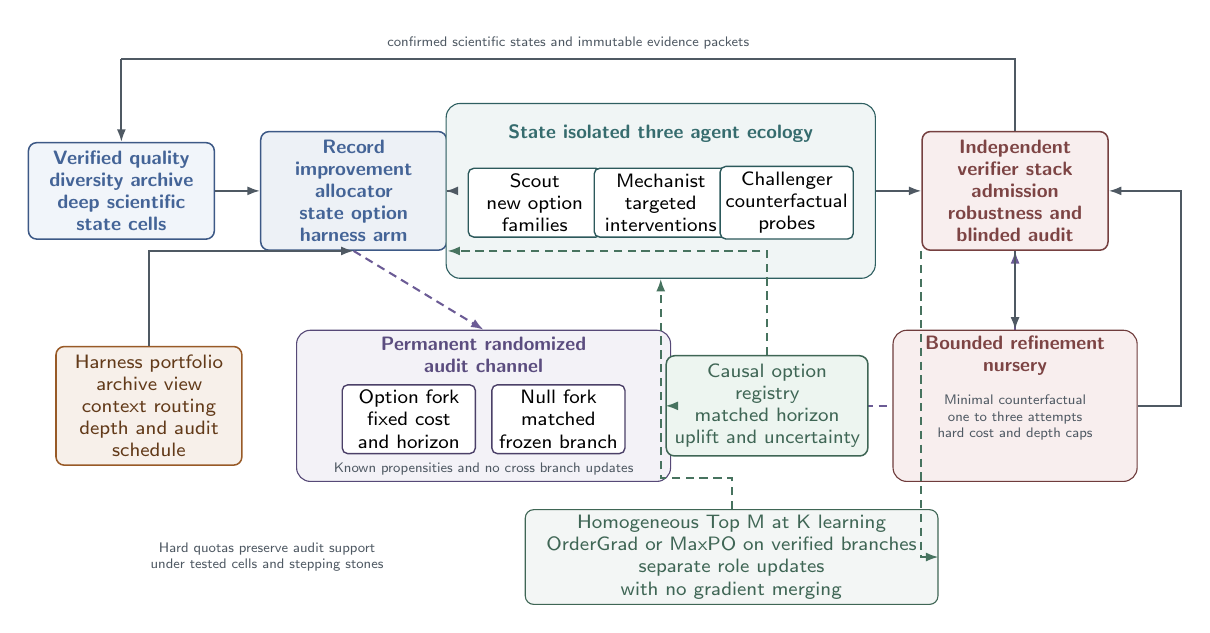
\begin{tikzpicture}[
  x=1cm,
  y=1cm,
  font=\sffamily\scriptsize,
  box/.style={rounded corners=3pt, align=center, minimum height=1.05cm,
    text width=2.15cm, inner sep=3pt, line width=0.55pt},
  smallbox/.style={rounded corners=2pt, align=center, minimum height=0.72cm,
    text width=1.55cm, inner sep=2pt, line width=0.5pt},
  flow/.style={-{Latex[length=1.6mm,width=1.15mm]}, draw=linegray, line width=0.7pt},
  audit/.style={-{Latex[length=1.6mm,width=1.15mm]}, draw=auditpurple, densely dashed, line width=0.75pt},
  update/.style={-{Latex[length=1.6mm,width=1.15mm]}, draw=memorygreen!90!black, densely dashed, line width=0.75pt}
]

\node[box, draw=searchblue!80!black, fill=statefill, text=searchblue!90!black,
  font=\sffamily\scriptsize\bfseries] (archive) at (0.7,4.45)
  {Verified quality diversity archive\\deep scientific state cells};

\node[box, draw=searchblue!80!black, fill=searchblue!10, text=searchblue!90!black,
  font=\sffamily\scriptsize\bfseries] (allocator) at (3.65,4.45)
  {Record\\improvement\\allocator\\state option\\harness arm};

\node[draw=policyteal!75!black, fill=policyteal!8, rounded corners=5pt,
  minimum width=5.45cm, minimum height=2.22cm] (ecology) at (7.55,4.45) {};
\node[font=\sffamily\scriptsize\bfseries, text=policyteal!85!black]
  at (7.55,5.18) {State isolated three agent ecology};
\node[smallbox, draw=policyteal!70!black, fill=white] (scout) at (5.95,4.30)
  {Scout\\new option families};
\node[smallbox, draw=policyteal!70!black, fill=white] (mechanist) at (7.55,4.30)
  {Mechanist\\targeted interventions};
\node[smallbox, draw=policyteal!70!black, fill=white] (challenger) at (9.15,4.30)
  {Challenger\\counterfactual probes};

\node[box, draw=verifyred!85!black, fill=rlfill, text=verifyred!90!black,
  font=\sffamily\scriptsize\bfseries] (verifier) at (12.05,4.45)
  {Independent verifier stack\\admission robustness and blinded audit};

\draw[flow] (archive.east) -- (allocator.west);
\draw[flow] (allocator.east) -- (ecology.west);
\draw[flow] (ecology.east) -- (verifier.west);

\coordinate (topright) at (12.05,6.12);
\coordinate (topleft) at (0.70,6.12);
\draw[draw=linegray, line width=0.7pt] (verifier.north) -- (topright) -- (topleft)
  node[midway, above, font=\sffamily\tiny, text=linegray]
  {confirmed scientific states and immutable evidence packets};
\draw[flow] (topleft) -- (archive.north);

\node[box, draw=harnessorange!85!black, fill=harnessorange!10,
  text=harnessorange!55!black] (harness) at (1.05,1.72)
  {Harness portfolio\\archive view\\context routing\\depth and audit\\schedule};
\draw[flow] (harness.north) |- (allocator.south);

\node[draw=auditpurple!80!black, fill=auditpurple!8, rounded corners=5pt,
  minimum width=4.75cm, minimum height=1.92cm] (forkbg) at (5.30,1.72) {};
\node[font=\sffamily\scriptsize\bfseries, text=auditpurple!85!black, align=center]
  at (5.30,2.37) {Permanent randomized\\audit channel};
\node[smallbox, draw=auditpurple!70!black, fill=white] (optionfork) at (4.35,1.55)
  {Option fork\\fixed cost and horizon};
\node[smallbox, draw=auditpurple!70!black, fill=white] (nullfork) at (6.25,1.55)
  {Null fork\\matched frozen branch};
\node[font=\sffamily\tiny, text=linegray] at (5.30,0.92)
  {Known propensities and no cross branch updates};
\draw[audit] (allocator.south) -- (forkbg.north);
\draw[audit] (forkbg.east) -| node[pos=0.60, below, font=\sffamily\tiny]
  {verified descendant maxima} (verifier.south);

\node[box, draw=memorygreen!80!black, fill=memoryfill,
  text=memorygreen!80!black, text width=2.35cm] (memory) at (8.90,1.72)
  {Causal option\\registry\\matched horizon\\uplift and uncertainty};
\draw[update] (forkbg.east) -- (memory.west);
\draw[update] (memory.north) |- (allocator.south east);

\node[draw=verifyred!80!black, fill=rlfill, rounded corners=5pt,
  minimum width=3.10cm, minimum height=1.92cm] (nurserybg) at (12.05,1.72) {};
\node[font=\sffamily\scriptsize\bfseries, text=verifyred!90!black, align=center]
  at (12.05,2.36) {Bounded refinement\\nursery};
\node[font=\sffamily\tiny, align=center, text=linegray] at (12.05,1.57)
  {Minimal counterfactual\\one to three attempts\\hard cost and depth caps};
\draw[flow] (verifier.south) -- (nurserybg.north);
\draw[flow] (nurserybg.east) -- ++(0.55,0) |- (verifier.east);

\node[draw=memorygreen!80!black, fill=memorygreen!7, rounded corners=3pt,
  align=center, text=memorygreen!80!black, text width=5.10cm,
  minimum height=0.72cm, inner sep=2pt] (learning) at (8.45,-0.20)
  {Homogeneous Top M at K learning\\OrderGrad or MaxPO on verified branches\\separate role updates with no gradient merging};
\draw[update] (verifier.south west) |- (learning.east);
\draw[update] (learning.north) -- ++(0,0.40) -| (ecology.south);

\node[font=\sffamily\tiny, text=linegray, align=center] at (2.55,-0.20)
  {Hard quotas preserve audit support\\under tested cells and stepping stones};

\end{tikzpicture}
}
\caption{EVOLVE joins four feedback loops through independently verified evidence. The production loop seeks record improvement. The randomized audit loop identifies option effects. The role loop updates isolated policies from homogeneous descendant groups. The archive loop preserves locally strong and scientifically distinct states.}
\label{figframework}
\end{figure}

\subsection{Scientific State Cells}
\label{secstates}

The archive stores scientific states rather than surface realizations. A versioned descriptor
\begin{equation}
\phi_v(x,e)
=
\left(
\phi_v^{\mathrm{beh}}(x,e),
\phi_v^{\mathrm{mech}}(x,e),
\phi_v^{\mathrm{con}}(x,e)
\right)
\label{eqfingerprint}
\end{equation}
combines controlled response vectors, mechanistic structure, and active constraint signatures. Text similarity may support retrieval but never defines identity. The map $q_v$ assigns a descriptor to a cell $c=q_v(\phi_v(x,e))$. Descriptor and cell versions remain frozen within each allocation epoch. Reindexing occurs only at synchronization barriers and never rewrites the provenance of earlier evidence.

Each cell is deep rather than elitist. It retains a confirmed quality representative, an option value representative, and a small randomized stepping stone reservoir. Descriptor uncertainty is represented by soft cell membership and repeated confirmation. Local competition compares confirmed lower confidence values only among nearby scientific states. A global record holder is retained separately and cannot be evicted.

State identity and transition identity are intentionally different. Several realizations can map to the same scientific state. The same proposal operator can also lead to different states. EVOLVE therefore keys transition evidence by the ordered pair $(c,o)$, where $c$ is a scientific state cell and $o$ is an option family. This pair is the basic allocation unit. It preserves mechanistically different routes without mistaking surface novelty for scientific diversity.

A fixed coverage quota reserves allocations for empty or under tested cells and for the stepping stone reservoir. The quota is a hard budget constraint rather than a novelty reward. Within the remaining budget, cells compete only through posterior record improvement. Quality diversity therefore protects search support without altering Eq.~\eqref{eqobjective}. This design follows the local competition principle of MAP-Elites while accounting for uncertain descriptors and scores \citep{mouret2015,flageat2023}.

\subsection{Temporally Extended Causal Options}
\label{secoptions}

An option is a temporally extended scientific transformation
\begin{equation}
o
=
\left(
I_o,
\pi_o,
\beta_o,
H_o
\right).
\label{eqoption}
\end{equation}
Here $I_o$ is the set of cells in which the option may begin, $\pi_o$ is its internal proposal policy, $\beta_o$ is its termination rule, and $H_o$ is its maximum branch cost. This extends the options formalism from temporal abstraction to scientific search \citep{sutton1999,bacon2017}.

Let $a\in\Agents$ denote an agent role and let $h\in\Harness$ denote a harness. Launching $(c,a,h,o)$ creates an isolated descendant branch. For fixed horizon $H$, define
\begin{equation}
Z_H(c,a,h,o)
=
\max\left(
M_e,
\max_{x\in\Data_H(c,a,h,o)}
\lcb_d(x,e_x)
\right),
\label{eqdescendantmax}
\end{equation}
where $M_e$ is the incumbent frozen at the start of epoch $e$ and $\Data_H$ contains admitted descendants reached before the branch cost reaches $H$. The record gain is
\begin{equation}
G_H(c,a,h,o)
=
\pos{Z_H(c,a,h,o)-M_e}.
\label{eqrecordgain}
\end{equation}
This outcome gives credit to an option that opens a productive basin even when its first transition is only a stepping stone.

EVOLVE separates three quantities. Immediate effect concerns the first transition. Branch effect concerns the full $H$ step descendant maximum. Memory mediated effect concerns later retrieval of a stored option. The causal registry uses only the branch effect
\begin{equation}
\tau_H(c,a,h,o)
=
\mathbb E\!\left[
G_H(c,a,h,o)-G_H(c,a,h,o_0)
\ \middle|\ 
c,a,h,e
\right],
\label{eqoptioneffect}
\end{equation}
where $o_0$ is a matched null continuation. Equation~\eqref{eqoptioneffect} measures the causal effect of a search intervention on discovery. It does not claim that the option identifies a causal law in the scientific domain.

\subsection{Randomized Audit Forks and Causal Option Memory}
\label{secaudit}

Adaptive allocation favors apparent winners and cannot by itself identify option effects. EVOLVE therefore maintains a permanent randomized audit channel. At the beginning of epoch $e$, the agent checkpoints, archive version, descriptor map, verifier version, incumbent threshold, and horizon are frozen. A selected state is cloned into isolated branches. Entire branches are assigned to the option or its matched null with known propensity $p_i(o)$ bounded below by $p_{\min}>0$. Both branches receive the same cost and horizon. Descendants, memory, and parameter updates remain quarantined until the audit closes.

For $n$ audit forks, a basic inverse propensity estimate is
\begin{equation}
\widehat\mu_H(o)
=
\frac{1}{n}
\sum_{i=1}^{n}
\frac{\ind\{O_i=o\}G_{H,i}}{p_i(o)},
\qquad
\widehat\tau_H(o)
=
\widehat\mu_H(o)-\widehat\mu_H(o_0).
\label{eqipw}
\end{equation}
Assignments may depend on the logged history before the fork. Positivity and branch isolation preserve identification. Effect estimates remain local to the audited cell, role, harness, policy version, verifier version, and horizon. Evidence is pooled only through an explicit hierarchical model that exposes its assumptions.

The causal option registry $\Registry_t$ stores evidence records rather than free form lessons. Each record contains the intervention and null versions, initiation cell, role and harness, frozen checkpoint, propensity, cost, horizon, verifier version, descendant outcome distribution, effect estimate, uncertainty sequence, replication count, and expiration rule. Promotion requires a positive contextual lower confidence value in independently closed audit blocks. A natural language synthesis of several records is treated as a new intervention and must earn its own evidence. Retrieval also retains a randomized no memory audit arm.

This registry prevents feasibility gains from being mistaken for scientific tail gains. It also prevents a frequently retrieved option from appearing useful merely because it received more opportunities. Sparse records are compared through threshold posteriors. When outcome tails are heavy and enough block maxima exist, Quantile of Maxima offers a distribution light robust comparator \citep{baudry2022}.

\subsection{Posterior Record Improvement Scheduling}
\label{secscheduler}

An allocation arm is
\begin{equation}
x
=
(c,a,o,h,H,C),
\label{eqarm}
\end{equation}
where $C$ is its total branch cost. Let $Z_x$ denote its verified descendant maximum and let $\mathcal P_t$ be the joint posterior over arm outcomes. For a nonadaptive portfolio $S$, posterior expected record improvement is
\begin{equation}
\mathcal I_t(S)
=
\mathbb E_{\mathcal P_t}\!\left[
\pos{\max_{x\in S}Z_x-M_t}
\ \middle|\ 
\Data_t
\right].
\label{eqportfolio}
\end{equation}
The joint posterior is important because descendants from nearby cells and related agents can be strongly correlated. Redundant arms have little marginal value even when each arm looks strong in isolation.

If the predictive outcomes are conditionally independent with CDFs $F_{x,t}$, Eq.~\eqref{eqportfolio} becomes
\begin{equation}
\mathcal I_t(S)
=
\int_{M_t}^{U}
\left[
1-
\prod_{x\in S}F_{x,t}(z)
\right]
\,dz.
\label{eqrecordintegral}
\end{equation}
For $n$ equal cost copies of one arm, let $p_t(x,u)=\Pr(Z_x\geq u\mid\Data_t)$. Then
\begin{equation}
\mathcal I_t(\{x\}^{n})
=
\int_{M_t}^{U}
\left[
1-\left(1-p_t(x,u)\right)^n
\right]
\,du.
\label{eqthreshold}
\end{equation}
Beta posteriors on a moving threshold grid make Eq.~\eqref{eqthreshold} usable with sparse evidence. Admission mass and admitted score tails are modeled separately. This avoids fitting a fragile mean model to the part of the distribution that determines discovery.

The exact finite horizon control problem is
\begin{equation}
V(\Data,M,b)
=
\max_{x\,\mid\,C_x\leq b}
\mathbb E\!\left[
V\!\left(
\Data\cup\Data_x,
\max(M,Z_x),
b-C_x
\right)
\ \middle|\ 
\Data
\right],
\label{eqbellman}
\end{equation}
with $V(\Data,M,0)=M$. Posterior rollouts approximate Eq.~\eqref{eqbellman}. A cheaper batch rule greedily adds the arm with the largest conditional marginal value in Eq.~\eqref{eqportfolio}. Section~\ref{sectheory} shows why this greedy rule is principled for a fixed unit cost portfolio.

Three hard quotas precede exploitation. One preserves the randomized audit support. One covers empty and under tested scientific cells. One preserves each agent role and provisional harness during cold start. The remaining resources maximize posterior record improvement. Diversity and information gain are therefore constraints on allocation rather than additions to reward.

\subsection{The Harness as an Arm}
\label{secharness}

A harness specifies an archive view, context assembly rule, role routing rule, breadth and depth schedule, resource envelope, and verification schedule. It changes the transition distribution and is therefore part of the intervention. EVOLVE never assumes one fixed harness is universally best. This follows recent evidence that discovery harness rankings vary across model and problem pairs and that early progress can guide online allocation \citep{gupta2026}.

The scheduler selects the joint arm $(c,a,o,h)$ rather than choosing a harness once before discovery. A factorized posterior shares statistical strength across the main effects of cells, agents, options, and harnesses while retaining selected low order interactions. New harnesses enter through a capped probation portfolio. Budget matched pilot branches determine whether they receive more resources. The independent verifier remains fixed while harnesses compete, so a permissive internal approximation cannot redefine archive admission.

Harness allocation and option attribution remain separate. Production outcomes update the tail model used for scheduling. Randomized matched forks update the causal registry. A harness may have high absolute record value even when its causal difference from a close alternative is uncertain. Conversely, a positive local causal effect does not imply that the arm has the highest absolute chance of beating the current record.

\subsection{A Three Agent Discovery Ecology}
\label{secagents}

EVOLVE uses three complementary agent roles.

\paragraph{Scout}
The Scout proposes new option families, representation changes, and transitions toward remote or empty scientific cells. Each proposal includes initiation conditions, a predicted descriptor shift, a termination rule, and a condition that would refute its rationale.

\paragraph{Mechanist}
The Mechanist applies targeted interventions to active constraints and invariants. It seeks options whose first transition may be modest but whose verified descendants have high record value.

\paragraph{Challenger}
The Challenger searches for counterexamples, boundary cases, and minimal counterfactual refinements. It never grades its own output. All promotion decisions belong to the independent verifier stack.

The roles form a state isolated ensemble rather than a statistically independent ensemble. They may share a frozen foundation model, but each role owns a separate adapter, optimizer state, random stream, private working memory, and retrieval view. Raw transcripts never cross roles. Communication uses immutable public evidence packets and occurs only at synchronization barriers. Heterogeneous foundation models may strengthen the ecology, but the framework makes no independence claim from parameter separation alone.

Each role receives a minimum allocation quota. The remaining role allocation is selected by posterior record improvement. This keeps the Challenger from becoming a universal gatekeeper and keeps early exploitation from extinguishing the Scout. Evidence may be shared after verification. Gradients are never shared or merged.

\subsection{Exact Learning from Descendant Maxima}
\label{seclearning}

Learning uses the same descendant outcome that guides search. Fix a homogeneous context
\begin{equation}
u
=
(c,a,o,h,H,M_e,\theta_e)
\label{eqcontext}
\end{equation}
and draw $N>K$ independent option trajectories from one frozen policy snapshot. Let their verified descendant gains be $G_1,\ldots,G_N$. For sorted gains $G_{(1,K)}\leq\cdots\leq G_{(K,K)}$, define the order statistic objective
\begin{equation}
J_{K,\alpha}(\theta\mid u)
=
\mathbb E\!\left[
\sum_{j=1}^{K}\alpha_jG_{(j,K)}
\right].
\label{eqorderobjective}
\end{equation}
Pure Max at $K$ sets $\alpha_K=1$. Top $m$ at $K$ spreads equal mass over the largest $m$ ranks. The latter can reduce sensitivity to one noisy extreme while remaining aligned with upper tail discovery.

For each sample $i$, let $q_i^{\alpha}$ be the average rank weighted value of all size $K$ subsets containing $i$. Let $v_i^{-,\alpha}$ be the corresponding average over all size $K$ subsets that exclude $i$. The exact OrderGrad advantage is
\begin{equation}
a_i^{\alpha}
=
q_i^{\alpha}-v_i^{-,\alpha},
\qquad
\widehat g_{\mathrm{OG}}
=
\frac{K}{N}
\sum_{i=1}^{N}
a_i^{\alpha}
\nabla_{\theta}\log\pi_{\theta}(\xi_i\mid u).
\label{eqordergrad}
\end{equation}
OrderGrad proves that Eq.~\eqref{eqordergrad} is unbiased for the finite sample objective in Eq.~\eqref{eqorderobjective} under its sampling assumptions \citep{parmas2026}. For pure Max at $K$, MaxPO supplies an exactly centered leave two out expected improvement advantage and can replace the top rank OrderGrad transformation \citep{takashiro2026}.

The guarantee applies only within groups that share the cell, role, option, harness, horizon, cost stratum, policy version, and frozen record threshold. EVOLVE never pools heterogeneous parents or policy snapshots into one exact gradient group. Each role updates only its own adapter. The frozen base and other role adapters remain unchanged. Arbitrary advantage clipping, nonlinear normalization, and cross group standardization are omitted when exactness is required. Only completed and independently verified branches enter this learning channel.

\subsection{Independent Verification and Bounded Refinement}
\label{secverification}

One public scalar is insufficient for archive admission. EVOLVE separates a navigation score from a verifier stack containing admissibility checks, the primary scientific measure, controlled perturbation responses, repeated confirmation when outcomes are stochastic, and a blinded audit view. The archive ranks admitted candidates by a simultaneous lower confidence value across the prespecified views. Agents receive a compact certificate after a branch closes, while blinded challenge content remains hidden.

A provisional candidate with a localized and actionable diagnosis may enter a bounded refinement nursery. Each ticket receives one to three attempts, a fixed cost ceiling, a maximum depth of two, and no recursive reentry. The Challenger proposes the smallest counterfactual change that could alter the verifier decision. Every revised candidate returns to the blinded verifier as a new immutable evidence packet. Only a confirmed improvement can enter the archive, option registry, or policy learning groups.

Refinement is itself a conditional option. In the audit channel, eligible provisional packets are randomized between refinement and an equal cost fresh continuation. This estimates contextual refinement uplift without comparing two populations selected by different rules. Nursery cost is charged in full and its total share is capped before record seeking begins.

\subsection{One Discovery Cycle}
\label{seccycle}

One synchronized epoch follows the steps below.

\begin{enumerate}
\item Freeze role checkpoints, archive and descriptor versions, verifier version, horizon set, and incumbent threshold.
\item Select frontier states from local quality representatives, under tested cells, option value representatives, and the stepping stone reservoir.
\item Form state, role, option, harness, horizon, and cost arms.
\item Reserve permanent audit, coverage, role, and harness support quotas.
\item Allocate the remaining portfolio by posterior marginal record improvement or Bellman rollouts.
\item Run production branches and randomized matched audit forks without cross branch updates.
\item Apply independent verification and route eligible provisional packets through the bounded nursery.
\item Merge confirmed scientific states and closed audit records at the synchronization barrier.
\item Update the causal option registry, the record posterior, and each isolated role adapter through their separate channels.
\end{enumerate}

The procedure stops when the resource budget is exhausted and returns the confirmed record holder with its lineage and evidence packet.

\section{Theoretical Properties}
\label{sectheory}

The theoretical claims concern finite horizon search effects and exact homogeneous learning groups. They do not imply universal harness superiority, statistical independence among agents, or causal truth inside the scientific domain.

\begin{assumption}[Frozen audit epoch]
Within an audit epoch, the starting state distribution, role checkpoints, archive view, descriptor map, harness, verifier, incumbent threshold, horizon, and cost are fixed.
\end{assumption}

\begin{assumption}[Positive randomized assignment]
Every compared option has a known logged branch assignment propensity bounded below by $p_{\min}>0$.
\end{assumption}

\begin{assumption}[Branch isolation]
One fork cannot change the candidates, memory, parameters, verifier state, or resources observed by another fork before the audit closes.
\end{assumption}

\begin{proposition}[Identification of finite horizon option value]
Under consistency and Assumptions 1 through 3, Eq.~\eqref{eqipw} is unbiased for the local finite horizon branch effect in Eq.~\eqref{eqoptioneffect}, conditional on the audited context.
\end{proposition}

\begin{proof}
Condition on the logged history immediately before assignment. For each potential branch outcome $G_{H,i}(o)$,
\begin{equation*}
\mathbb E\!\left[
\frac{\ind\{O_i=o\}G_{H,i}}{p_i(o)}
\ \middle|\ 
\mathcal F_{i-1}
\right]
=
G_{H,i}(o).
\end{equation*}
Consistency connects the observed outcome to the assigned potential outcome. Branch isolation removes interference. Averaging and subtracting the null arm yields the result.
\end{proof}

\begin{proposition}[Record acquisition is submodular]
Fix a posterior over any jointly distributed arm outcomes and a record $M$. The set function
\begin{equation*}
f(S)
=
\mathbb E\!\left[
\pos{\max_{x\in S}Z_x-M}
\right]
\end{equation*}
is normalized, monotone, and submodular. For unit costs, greedy marginal posterior record improvement obtains at least $1-1/e$ of the optimal fixed size nonadaptive portfolio.
\end{proposition}

\begin{proof}
For one realized outcome vector, the marginal value of adding arm $x$ is
\begin{equation*}
\pos{
Z_x-
\max\left(M,\max_{y\in S}Z_y\right)
}.
\end{equation*}
This quantity is nonnegative and can only decrease as $S$ grows. Expectation preserves normalization, monotonicity, and diminishing returns. The greedy guarantee follows from the classical cardinality constrained submodular maximization result.
\end{proof}

\begin{proposition}[Inherited exact upper rank gradient]
Fix a homogeneous context $u$. Assume independent on policy trajectories, bounded parameter independent verified gains, and valid differentiation under expectation. Then the OrderGrad estimator in Eq.~\eqref{eqordergrad} satisfies
\begin{equation*}
\mathbb E\!\left[\widehat g_{\mathrm{OG}}\right]
=
\nabla_{\theta}J_{K,\alpha}(\theta\mid u),
\qquad
\sum_{i=1}^{N}a_i^{\alpha}=0.
\end{equation*}
For the pure top rank objective, the centered MaxPO estimator inherits the corresponding Max at $K$ policy gradient guarantee.
\end{proposition}

\begin{proof}
This is the likelihood ratio OrderGrad result applied to verified descendant gains. Exchangeability lets the gradient of a size $K$ order statistic be written through include one values. The leave one out value is independent of the focal score term and has the same expectation. The finite subset counting identity centers the realized advantages. MaxPO obtains an equivalent centered construction for the pure maximum through its leave two out baseline.
\end{proof}

\begin{proposition}[Verified archive invariant]
If the global record holder is retained and replacement requires independent admission with a lower confidence value above the local incumbent, then the recorded sequence $M_t$ is nondecreasing.
\end{proposition}

\begin{proof}
Every update takes the maximum of the previous record and newly admitted lower confidence values. Removing nonrecord archive occupants cannot reduce this stored maximum.
\end{proof}

\section{Scope and Limitations}
\label{seclimitations}

Causal option values are local to their audited state cells, agents, harnesses, checkpoints, verifier versions, costs, and horizons. Transfer beyond that support is a modeling choice rather than an identified fact. A short horizon can undervalue delayed stepping stones, so EVOLVE maintains several horizon strata and a protected randomized reservoir. A descriptor map is only an operational approximation to scientific diversity. Freezing, uncertainty tracking, and versioned reindexing limit descriptor drift but cannot make the representation complete.

Independent verification is still proxy dependent. Simultaneous lower confidence scoring, blinded audit views, and repeated confirmation reduce extreme score noise but cannot establish truth outside the verifier's scope. The three roles are state isolated and may remain correlated through a common foundation model or evidence registry. Their residual correlation belongs in the joint record posterior. Finally, the framework guarantees neither open ended discovery nor global optimality. Its theory aligns finite budget allocation and learning with the verified record objective under explicit local assumptions.

\begin{thebibliography}{99}

\bibitem[Bacon et al.(2017)]{bacon2017}
Pierre-Luc Bacon, Jean Harb, and Doina Precup.
\newblock The option-critic architecture.
\newblock In \emph{Proceedings of the AAAI Conference on Artificial Intelligence}, 2017.

\bibitem[Baudry et al.(2022)]{baudry2022}
Dorian Baudry, Yoan Russac, and Emilie Kaufmann.
\newblock Efficient algorithms for extreme bandits.
\newblock In \emph{Proceedings of the International Conference on Artificial Intelligence and Statistics}, 2022.

\bibitem[Flageat and Cully(2023)]{flageat2023}
Manon Flageat and Antoine Cully.
\newblock Uncertain quality diversity with evaluation methodology and new methods for uncertain domains.
\newblock \emph{arXiv preprint 2302.00463}, 2023.

\bibitem[Gupta et al.(2026)]{gupta2026}
Akshat Gupta, Jermaine Lei, Alexander Lu, Gopala Anumanchipalli, and Leshem Choshen.
\newblock Automated discovery has no universally superior harness.
\newblock \emph{arXiv preprint 2607.18235}, 2026.

\bibitem[Mouret and Clune(2015)]{mouret2015}
Jean-Baptiste Mouret and Jeff Clune.
\newblock Illuminating search spaces by mapping elites.
\newblock \emph{arXiv preprint 1504.04909}, 2015.

\bibitem[Parmas et al.(2026)]{parmas2026}
Paavo Parmas, Yongmin Kim, Kohsei Matsutani, Shota Takashiro, Soichiro Nishimori, Takeshi Kojima, Yusuke Iwasawa, and Yutaka Matsuo.
\newblock OrderGrad and optimizing beyond the mean with order statistic policy gradient estimation.
\newblock \emph{arXiv preprint 2606.06096}, 2026.

\bibitem[Sutton et al.(1999)]{sutton1999}
Richard Sutton, Doina Precup, and Satinder Singh.
\newblock Between MDPs and semi-MDPs with a framework for temporal abstraction in reinforcement learning.
\newblock \emph{Artificial Intelligence}, 112, 1999.

\bibitem[Takashiro et al.(2026)]{takashiro2026}
Shota Takashiro, Soichiro Nishimori, Paavo Parmas, Yongmin Kim, Kohsei Matsutani, Gouki Minegishi, Yusuke Iwasawa, Takeshi Kojima, and Yutaka Matsuo.
\newblock On advantage estimates for Max at K policy gradients.
\newblock \emph{arXiv preprint 2606.06080}, 2026.

\end{thebibliography}

\end{document}
